\begin{sidewaysfigure*}
\thisfloatpagestyle{mylandscape}%
\rotatesidewayslabel%
\centering
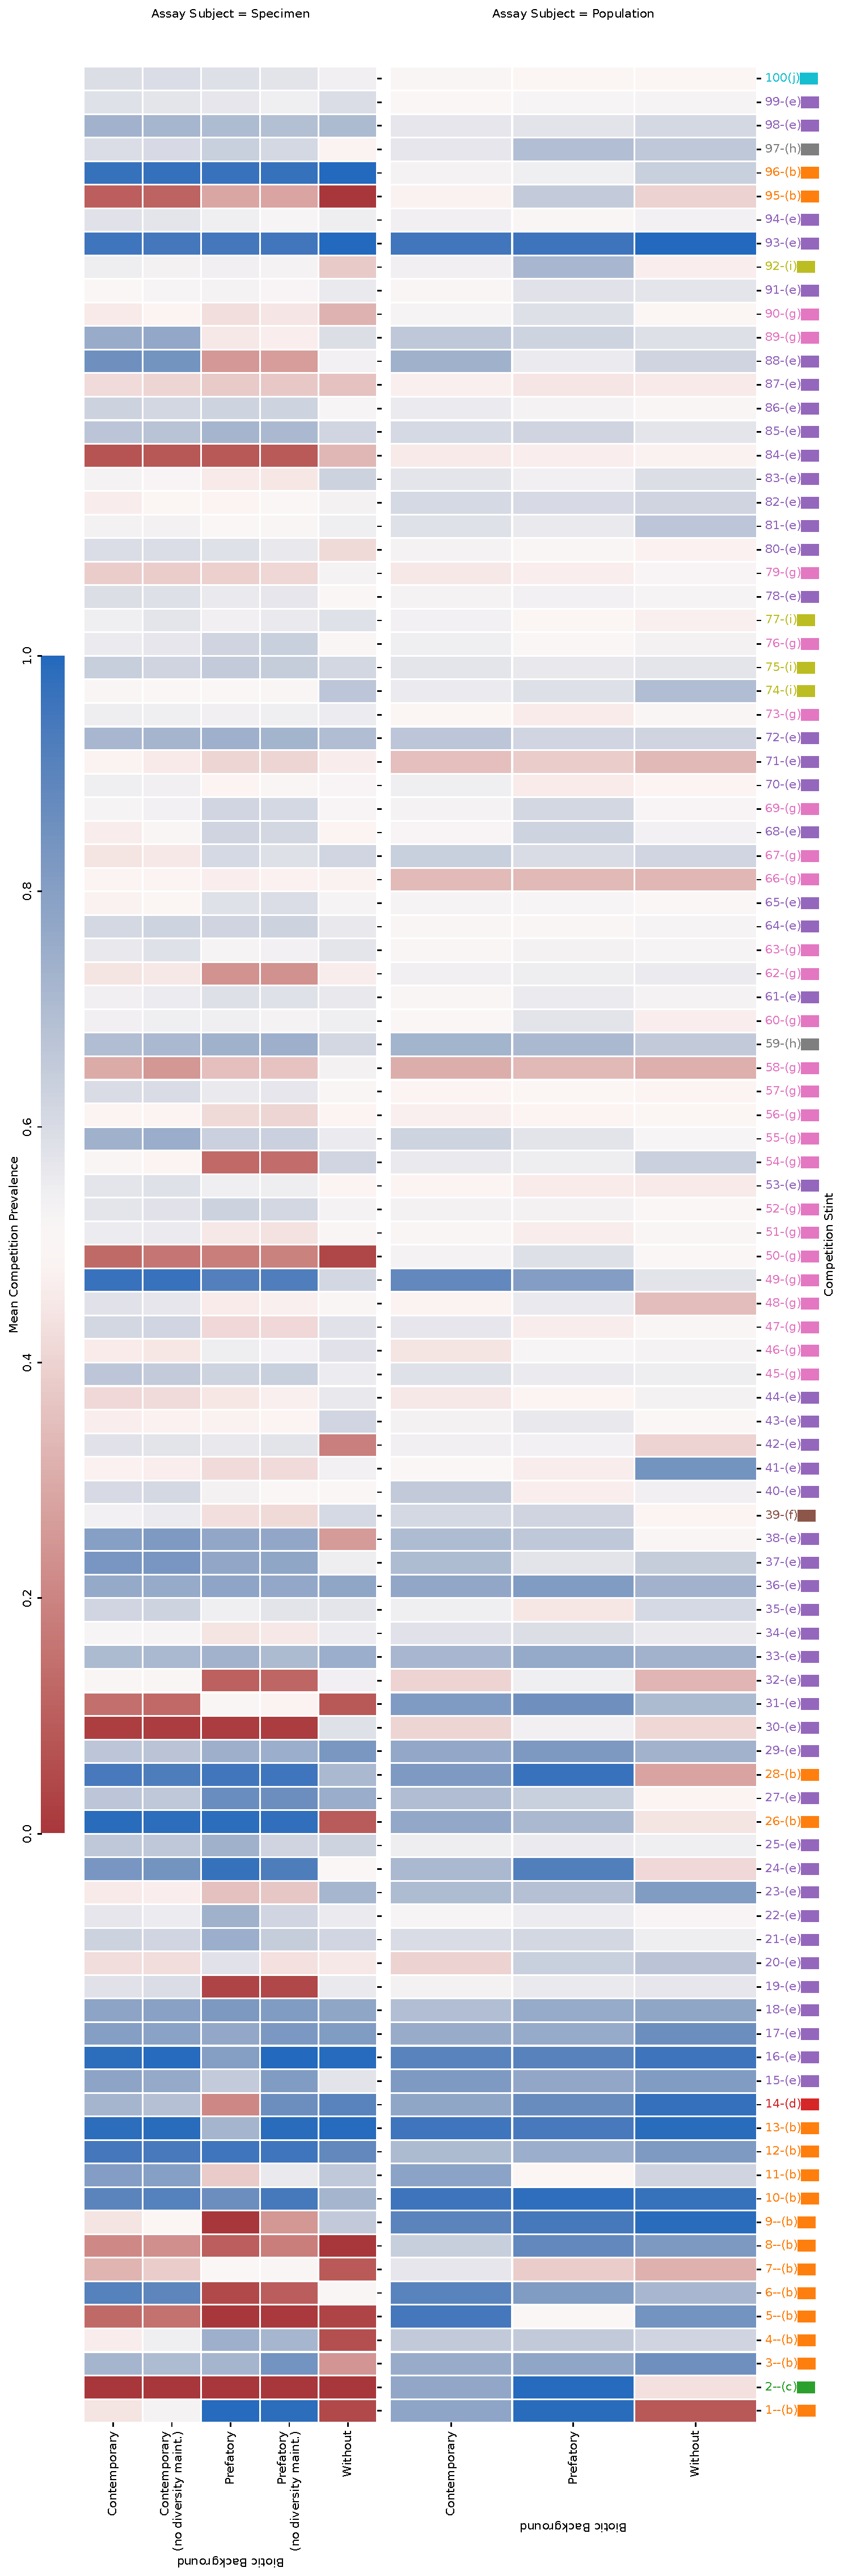
\includegraphics[width=\linewidth]{{submodule/dishtiny/binder/bucket=prq49/a=adaptation_assays+endeavor=16/teeplots/hue=mean-competition-prevalence+viz=facet-heatmap+x=biotic-background+y=competition-stint+ext=}}

\caption{
Mean end-state population composition of competition experiments.
Half (0.5) population composition corresponds to a neutral result, color mapped to white.
Blue indicates fitness gain compared to the previous stint and red indicates fitness loss.
Color coding and parentheticals of stint labels correspond to qualitative morph codes described in Table \ref{tab:morph_descriptions}.
Upper panel shows results for sampled focal strain genome, lower panel shows results for entire focal strain population.
See Figure \ref{fig:adaptation_assay_cartoon} for explanation of competition biotic backgrounds.
See Figure \ref{fig:mean_competition_prevalence_boxplot} for boxplot depiction of prevalence outcomes and Figure \ref{fig:mean_competition_prevalence_barplot} for bootstrapped confidence intervals on mean prevalence outcomes.
}
\label{fig:mean_competition_prevalence}
\end{sidewaysfigure*}
